\documentclass{article}

\usepackage[a4paper, margin=2cm]{geometry}
\usepackage{amsmath, amsfonts}
\usepackage{indentfirst}
\usepackage{graphicx}
\usepackage{minted}
\usepackage[pdfusetitle]{hyperref}

\title{34-2-3 Na Hroších pláních}
\author{Benjamin Swart}

\begin{document}

\maketitle

\section*{Úvod}

Snažíme se zjistit, jestli mají dva mnohoúhelníky průnik. Budu je označovat jako mnohoúhelník červený a modrý.

\section*{Algoritmus pro nalezení průniku dvou mnohoúhelníků a přímky}
\label{sec:findOnLine}

Pokud zjistíme (nebo se to domníváme), že se hledaný průnik nachází na nějakém specifickém řádku (tj. přímce rovnoběžnou s osou x), tak je jeho nalezení snadné.

Souřadnice vrcholů pospojujeme do seznamu úseček. Pro každou si uložíme, jestli je to strana červeného nebo modrého mnohoúhelníku.

Ze seznamu vybereme ty přímky, které náš řádek protínají a zeřadíme je podle souřadnice x tohoto průniku.

\begin{figure*}[h] \centering
    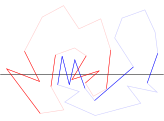
\includegraphics[width=10cm]{images/on-line.000.pdf}
\end{figure*}

S každou červenou čárou se změní, jestli jsme uvnitř červeného mnohoúhelníku. S modrou je to obdobně.

Procházíme tedy zleva doprava průniky řádku s hranami a invertujeme stavy obou mnohoúhelníků.

\begin{figure*}[h] \centering
    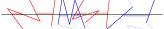
\includegraphics[width=10cm]{images/on-line.001.pdf}
\end{figure*}

Pokud narazíme na místo, kde jsme uvnitř obou mnohoúhelníků, tak jsme našli průnik. Jeden bod průniku bude zajisté v půly cesty mezi posledním zpracovaným bodem a bodem následujícím.

Tento algoritmus běží v \(O(n * log n)\) kvůli řazení.

\section*{Prvotní kontrola}

Existují tři kategorie vzájemných poloh mnohoúhelníků:

\begin{enumerate}
    \item Mnohoúhelníky se neprotínají
    \item Jeden mnohoúhelník leží uvnitř druhého
    \item Strany mnohoúhelníků se protínají
\end{enumerate}

Nejprve určíme nejvyšší a nejnižší souřadici Y vrcholu pro oba mnohoúhelníky. Získáme tak pro každý mnohoúhelník interval, ve kterém příslušný mnohoúhelník leží.

\begin{figure*}[h] \centering
    
\includegraphics[width=10cm]{images/interval.pdf}
\end{figure*}

Pokud se tyto intervaly neprotínají, tak se zajisté neprotínají ani mnohoúhelníky. Vracíme zápornou odpověď a program ukončujeme.

V případě, že jeden mnohoúhelník leží uvnitř druhého, tak se budou protínat i na libovolné řadě v průniku těchto intervalů. Jednu řadu vybereme (třeba veprostřed) a spustíme výše popsaný algoritmus.

\begin{figure*}[h] \centering
    
\includegraphics[width=10cm]{images/inside.pdf}
\end{figure*}

Pokud průnik najdeme, tak ho vrátíme a program ukončujeme. V případě, že průnik nenajdeme, tak máme jistotu, že jeden mnohoúhelník neleží uvnitř druhého a že se mnohoúhelníky buď neprotínají, nebo se někde kříží jejich strany.

\section*{Detekce křížících se stran}

Vytvoříme si seznam stran a uložíme je do jednoho seznamu. Ani si nemusíme pamatovat, kterému mnohoúhelníku náleží.

Vytvoříme si seznam událostí.

Budou v něm takovéto trojice:

\begin{minted}{cpp}
enum event_type { start, end };

struct event {
    int y;
    event_type type;
    edge *edge;
};
\end{minted}

Pro každou stranu vytvoříme dvě události: Jednu, která říká, že na souřadici \(min(y_1, y_2)\) začíná a jednu, která říká, že na souřadici \(max(y_1, y_2)\) končí.

Tento seznam seřadíme podle \(y\).

Nyní můžeme tento seznam procházet odzhora dolů a ukládat si seznam hran, které jsou právě aktivní. Když narazíme na událost typu \emph{start}, tak hranu do seznamu přídáme, a když narazíme na \emph{end}, tak ji naopak odebereme.

Po zpracování všech událostí pro danou souřadici y dostaneme reprezentaci všech hran na tomto řádku. Abychom si práci usnadnili, zvolíme pro seznam akuálních hran dobrou datovou strukturu. Použijeme red-black tree, který je v C++ implementován strukturou \emph{std::set}.

Je samozřejmě důležité tento strom podle něčeho seřadit. Seřadíme ho podle souřadnice x průniku s aktuálním řádkem. Pokud se hrany nebudou protínat, tak zůstane strom seřazený po celou dobu běhu algoritmu. Pokud se protínají, tak se strom rozbije jakmile se dostaneme za souřadici y jejich průniku. Musíme si tedy dobře ohlídat aby, takováto situace nenastala. Pokud takový bod odhalíme, tak máme skoro hotovo.

\begin{figure*}[h] \centering
    
\includegraphics[width=10cm]{images/line.000.pdf}
\end{figure*}

Aby se dvě strany mohly protnout, musí být v tomto stromě vedle sebe. Pokud mezi nimi leží jiná hrana, musela by se buď jedna ze stran nejprve protnout s ní, nebo by musela prostředí hrana nejprve zkončit.

\begin{figure*}[h] \centering
    
\includegraphics[width=10cm]{images/line.001.pdf}
\end{figure*}

Stačí tedy mít v každém okamžiku zkontrolované, zda se žádné sousední strany neprotínají. Jelikož se sousedství v seznamu může měnit jen v bezprostřední blízkosti nějaké změny, tak nám stačí provádět kontroly ve dvou případech:

\begin{enumerate}
    \item Pokud přidáváme hranu do seznamu, zkontrolujeme, zda se nekříží s jedním z jejích nových sousedů
    \item Pokud odebíráme hranu ze seznamu, tak zkontrolujeme, zda se její dva staří sousedi nekříží
\end{enumerate}

\begin{figure*}[h] \centering
    \includegraphics[width=10cm]{images/line.002.pdf}
    
\includegraphics[width=10cm]{images/line.003.pdf}
\end{figure*}

Pokud v jednom z těchto případů narazíme na křížení, víme, že se mnohoúhelníky protínají. Zbývá jen najít alespoň jeden bod průniku mnohoúhelníku.

Vypočítáme souřadnice průniku dotčených hran. Nějaký průnik určitě najdeme buď nad nebo pod tímto bodem. Najdeme si nejbližší souřadici y vyskytující se ve vstupních datech ve směru nahoru i dolů. Vypočítáme souřadnici v půli cesty z souřadnice y křížení k těmto souřadicím.

\begin{figure*}[h] \centering
    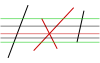
\includegraphics[width=10cm]{images/search.pdf}
    \linebreak
    Překřížení hran (červené), nejbližší použité souřadnice y (zelené), a řady v půli cesty mezi nimi (černé)
\end{figure*}

Na obou těchto řádcích spustíme výše uvedený \hyperref[sec:findOnLine]{Algoritmus pro nalezení průniku dvou mnohoúhelníků a přímky}. Jeden z nich určitě průnik najde.

Pokud se dostaneme na konec dokumentu bez jakéhokoliv překřížení, tak odpovídáme záporně.

\end{document}

